\documentclass[journal]{IEEEtran}
\usepackage{xcolor}
\usepackage{cite}
\usepackage{amsmath,amssymb,amsfonts}
\usepackage{algorithm}
\usepackage{algpseudocode}
%\usepackage{algorithmic}
\usepackage{graphicx}
\usepackage{textcomp}
\usepackage{graphicx}
%\usepackage{caption}
\usepackage{subcaption}
\usepackage[hyphens]{url}
\usepackage{placeins}

% correct bad hyphenation here
% \hyphenation{op-tical net-works semi-conduc-tor}

\begin{document}

\title{ELEC1601 Exercise 2 Lab Report}

\author{SID: 530157791, Lab Group: F12 19}

% make the title area
\maketitle


\begin{abstract}
The purpose of this lab was to delve into digital logic and control systems using an Arduino, a 7-segment display, and servo motors. We executed the simulation and coding on Tinkercad based on the provided tutorial and successfully transitioned the project to a physical setup in our week 5 lab session. This experience equipped me with a foundational understanding of 7-segment displays and servo motors, as well as the skills to manipulate them via Arduino programming.
\end{abstract}

\section{Introduction}
\IEEEPARstart{T}{he} purpose of this lab session was to have a deep understanding of basic electronics and microcontroller programming, particularly focusing on digital logic and hardware-software interaction. Key skills targeted for development included:
%purpose of this lab session was … (what you think we want you to learn/skills we want you to develop)

% Overview of learning outcomes and methods used.
In this lab, our focus was on teamwork, understanding digital logic, Arduino programming, circuit setup, and control logic. We utilized both software (Arduino IDE and TinkerCAD) and hardware (7-segment display and servo motors) tools to meet these objectives.

% Main methods for achieving the learning outcomes
\begin{itemize}
\item  \textbf{Software}: Used Arduino IDE for programming and TinkerCAD for virtual prototyping.
\item  \textbf{Hardware}: Employed a 7-segment display and servo motors, connected to an Arduino Uno.
\item  \textbf{Teamwork}: Maintained weekly meetings and code reviews for efficient collaboration.
\end{itemize}

% Summary of the final implementation and skills gained.
Our efforts improved our skills in teamwork and circuit designresulting in a successful multi-device setup. Key implementations include button-controlled 7-segment display transitions and servo motor positioning.

\section{Background}

Key components and their roles and real-world applications are outlined in the table below.

\begin{tabular}{|p{1.6cm}|p{3.5cm}|p{2.5cm}|}
\hline
\textbf{Component} & \textbf{Lab Use} & \textbf{Real-world Applications} \\
\hline
Arduino Uno\cite{ArduinoOfficialDocs} & Brain of system. Controls display, servos, button. & DIY, automation. \\
\hline
Wires & Connection medium. Connects components. & Circuits, power. \\
\hline
Computer with Arduino IDE\cite{ArduinoSoftware} & Enables Programming. Codes Arduino. & Software dev. \\
\hline
Resistors & Limits current. Current control. & Circuits. \\
\hline
7-Segment Display & Displays numbers. Shows numbers. & Clocks, signage. \\
\hline
Servo Motors (x2) & Controls position. Shaft positioning. & Robotics. \\
\hline
Button & Switch mechanism. User control. & Appliances. \\
\hline
TinkerCAD & Online testing tool. Prototyping. & Education. \\
\hline
\end{tabular}





\section{Method}
\subsection{Part I}

% Insert circuit diagram
\begin{figure}[h]
\centering
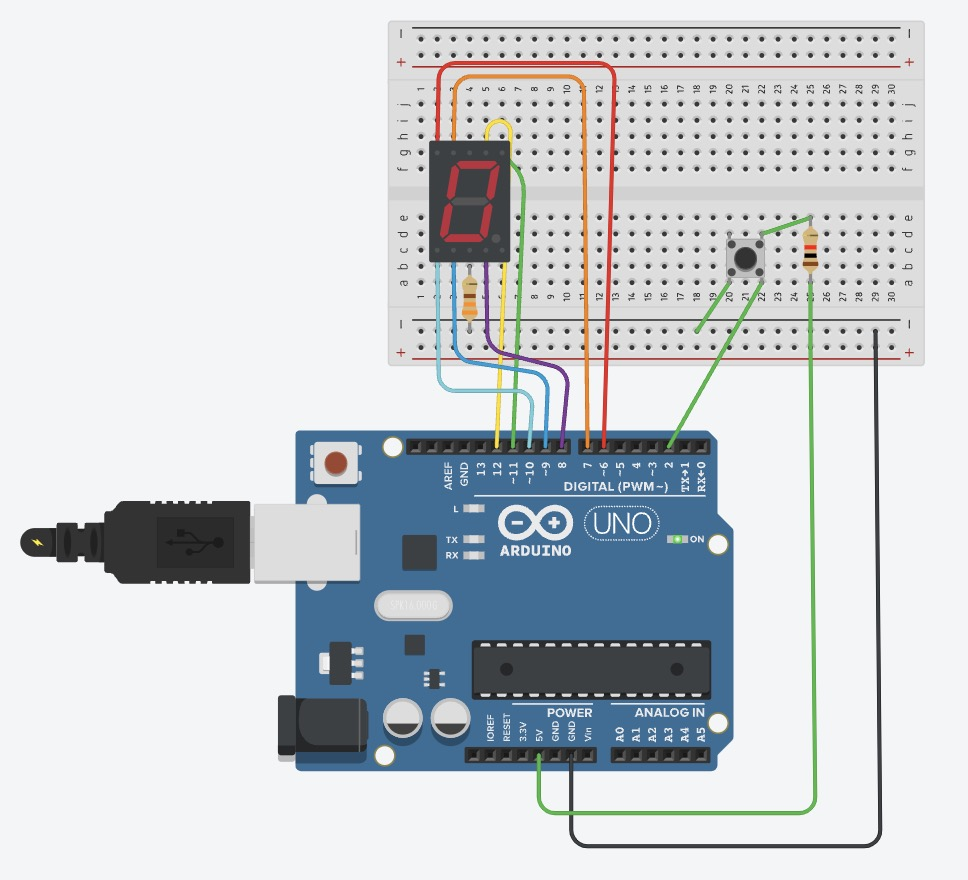
\includegraphics[width=0.3\textwidth]{images/Part1_circuits.jpg}
\caption{Circuit diagram for Part I}
\label{fig:circuit_part1}
\end{figure}

% Describe the circuit you created in Part I
The circuit we created for Part I, as shown in Figure~\ref{fig:circuit_part1}, includes a 7-segment display contains 7 segments. Each segment is controlled independently by pin6 - pin12 on Arduino Uno, corresponding to segments A to G of the display. A resistor of 330-ohms is connected in series with each segment.
In addition, a button is connected to pin 2 (interrupt 0). When the button is pressed, the voltage on pin 2 changes from 1 to 0 (FALLING).
% Describe your pseudocode with a LaTeX algorithm environment
\begin{algorithm}
\caption{Shortened Pseudocode for 7-Segment Counter}\label{alg:7segment_counter}
\begin{algorithmic}[1]
\State Init Booleans \( A, B, C, D, E, F, G \), \( \text{count} = 0 \)
\State Configure pins; Attach FALLING interrupt to pin 2 with handler \( x \)

\Procedure{setup}{}
    \State Init serial at 9600 bps
\EndProcedure

\Procedure{loop}{}
    \State Print pin 2 state; Update \( A, B, C, D, E, F, G \) based on \( \text{count} \)
    \State Write to pins; Delay 500 ms
\EndProcedure

\Procedure{x}{}
    \State \( \text{count} = (\text{count} + 1) \mod 10 \)
\EndProcedure
\end{algorithmic}
\end{algorithm}

% Explain what this pseudocode does
The pseudocode in Algorithm~\ref{alg:7segment_counter} controls a 7-segment display with an Arduino Uno.
\begin{itemize}
    \item \textbf{Init:} Boolean variables \( A, B, C, D, E, F, G \) and \( \text{count} \) initialized.
    
    \item \textbf{Pins:} Pin 2 as INPUT for button; pins 6-12 as OUTPUT for segments \( A-G \).
    
    \item \textbf{Interrupt:} Attached to pin 2 to trigger function \( x \) on button press.
    
    \item \textbf{Loop:} 
    \begin{itemize}
        \item Debugs pin 2 state.
        \item Updates \( A-G \) based on \( \text{count} \).
        \item Writes to Arduino pins.
        \item 500-ms delay.
    \end{itemize}

    \item \textbf{Function \( x \):} Increments \( \text{count} \) mod 10, updates display.
\end{itemize}

% Design decisions
\textbf{Design Decisions:}

\begin{itemize}
    \item \textbf{Pin Selection:} Pins 6 to 12 were chosen as OUTPUT pins for segments \( G \) to \( A \) due to their proximity on the Arduino board, facilitating easier wiring. Pin 2 was chosen as the INPUT pin for the button because it supports interrupts, allowing for more efficient button press detection.
    
    \item \textbf{Use of Interrupts:} Interrupts were used to detect button presses, allowing the program to avoid constantly polling the button's state. 
    
    \item \textbf{Modular Counting:} The variable \( \text{count} \) was implemented with modular to reset after reaching 9, allowing the display to cycle back to 0.
\end{itemize}


% Limitations, Successes, Unexpected Results
\textbf{Observations:} The design successfully updates the 7-segment display on button press, utilizing modular arithmetic to back to 0 after 10 presses. 


\subsection{Part II}

\begin{figure}[H]
\centering
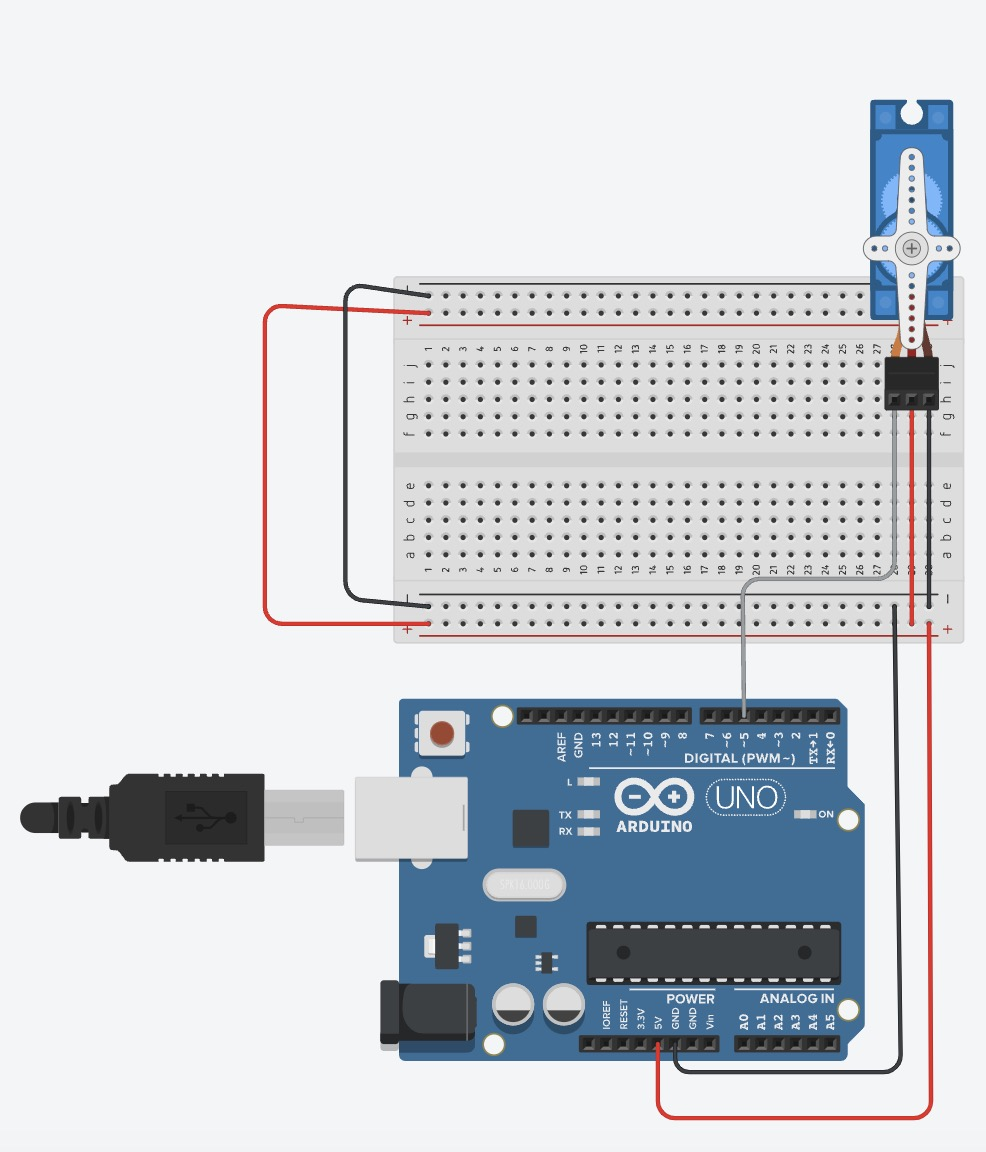
\includegraphics[width=0.2\textwidth]{images/Part2_circuits.jpg}
\caption{Circuit diagram for Part II}
\label{fig:circuit_part2}
\end{figure}

% Describe the circuit you created in Part II
The circuit we created for Part II, as shown in Figure~\ref{fig:circuit_part2}, includes a servo motor connected with Arduino uno.

% Describe your pseudocode with a LaTeX algorithm environment
\begin{algorithm}
\caption{Shortened Pseudocode for Servo Angle Manipulation}\label{alg:servo-short}
\begin{algorithmic}[1]
\State \textbf{Include} Servo library; Init \textit{servo, angle = 0}

\Function{Setup}{}
    \State Attach servo to pin 5
\EndFunction

\Function{Loop}{}
    \For{\textit{angle} from 0 to 150; step 30; wait 300 ms}
        \State Write \textit{angle} to servo
    \EndFor
    
    \For{\textit{angle} from 150 to 0; step -30; wait 300 ms}
        \State Write \textit{angle} to servo
    \EndFor
\EndFunction
\end{algorithmic}
\end{algorithm}



% Explain what this pseudocode does
The pseudocode outlined in Algorithm~\ref{alg:servo-short} controls a servo motor connected to pin 5 of the Arduino. The servo's angle increments from 0 to 150 degrees and decrements back to 0, each step separated by a 300-ms delay.

% Design Decisions
\textbf{Design Decisions}\\
Angle steps are set at 30 degrees and a 300-ms delay is used for a balance between speed and observation.

% Limitations, Successes, and Unexpected Results
\textbf{Limitations, Successes}\\
Limitation: Servo's 150-degree range despite 180-degree specs.Success: Effective servo angle control.

\subsection{Part III}
\begin{figure}[H]
\centering
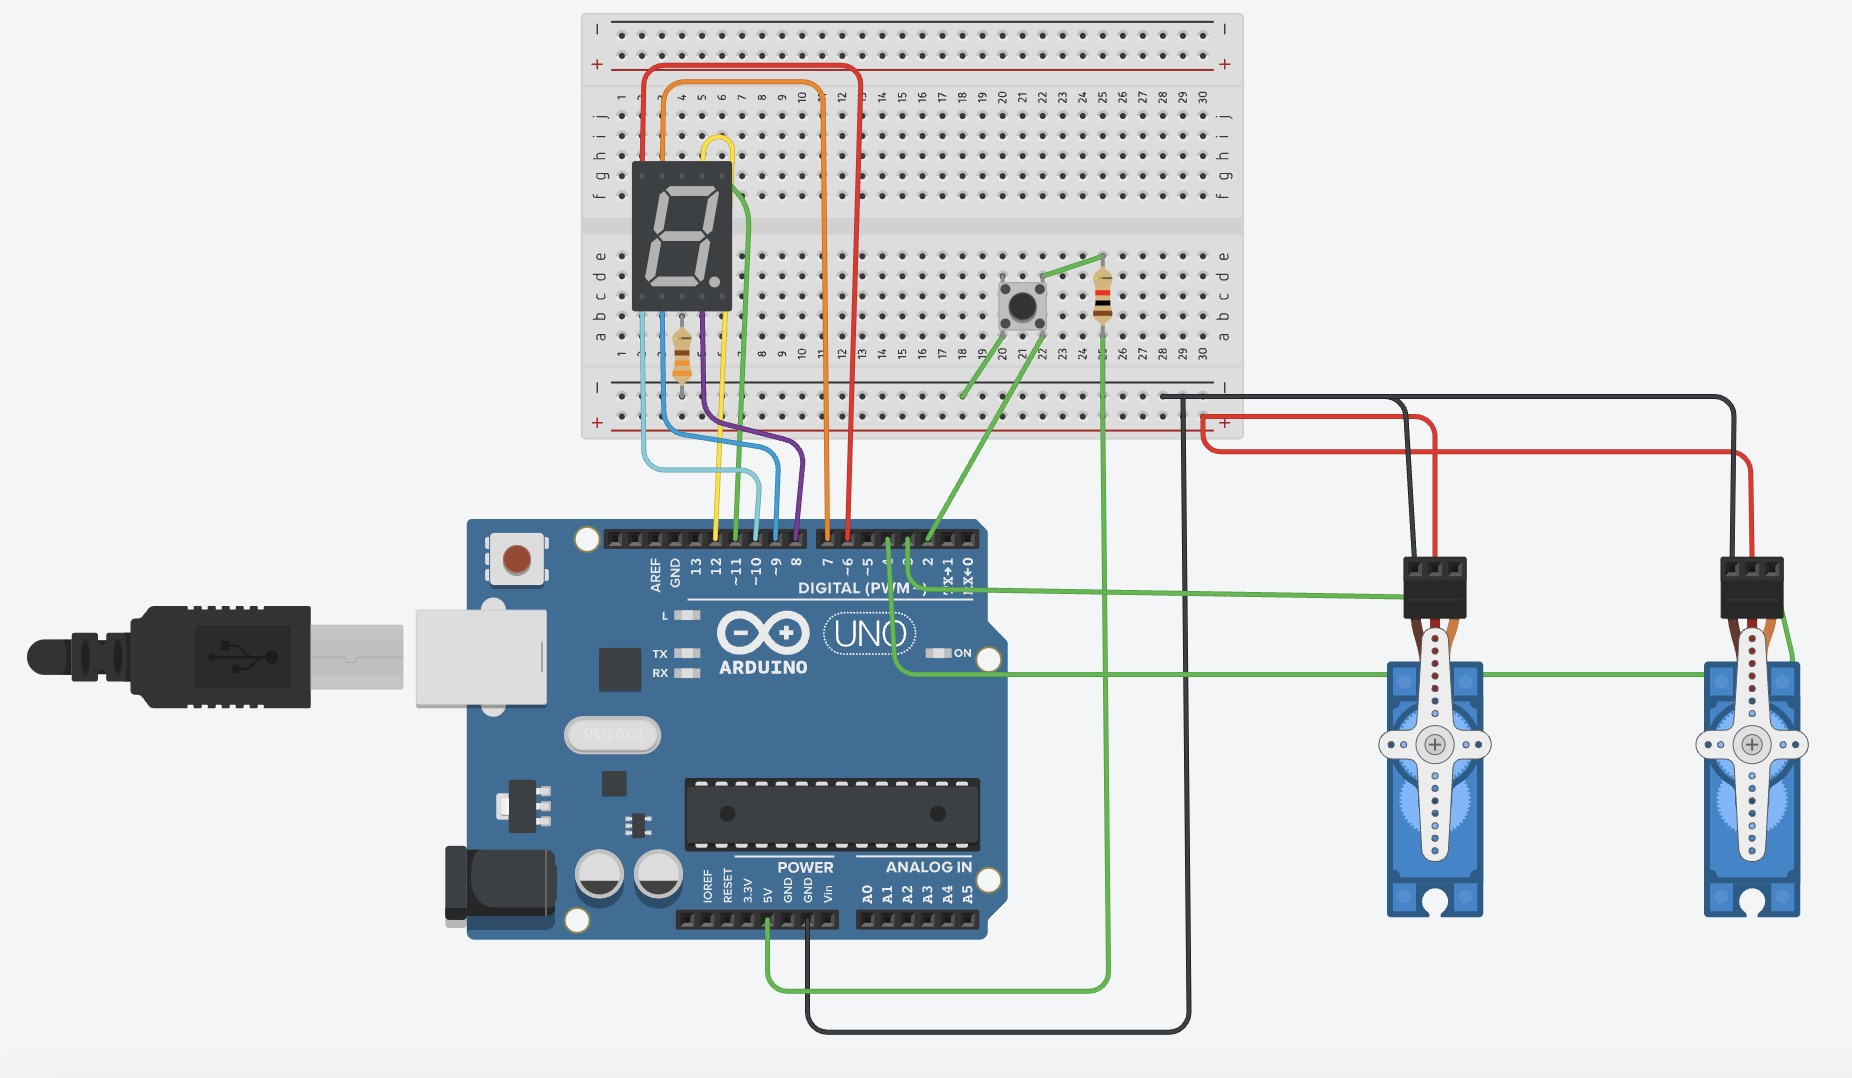
\includegraphics[width=0.46\textwidth]{images/Part3_circuits.jpg}
\caption{Circuit diagram for Part III}
\label{fig:circuit_part3}
\end{figure}

% Describe the circuit you created in Part II
The circuit we created for Part III, as shown in Figure~\ref{fig:circuit_part3}, includes a servo motor connected with Arduino uno.

% Describe your pseudocode with a LaTeX algorithm environment
\begin{algorithm}
\caption{Simplified Pseudocode for Part 3}\label{alg:7segment_servo}
\begin{algorithmic}[1]
\State Import Servo; Init servo1, servo2, pos1=0, pos2=180, count=0, A-G

\Procedure{Setup}{}
  \State Config pins; Attach interrupts; Attach servos; Init positions and Serial
\EndProcedure

\Procedure{Loop}{}
  \State Serial print pin 2; \Call{updateDisplay}{}; Update servo positions; Delay 500 ms
\EndProcedure

\Procedure{ISR}{}
  \State \( \text{count} = (\text{count} + 1) \mod 10 \); Update servos
\EndProcedure

\Procedure{updateDisplay}{}
  \State Update A-G; Write to 7-segment
\EndProcedure
\end{algorithmic}
\end{algorithm}

% Explain what this pseudocode does
The pseudocode outlined in Algorithm~\ref{alg:7segment_servo} controls a servo motor connected to pin 5 of the Arduino. The servo's angle increments from 0 to 150 degrees and decrements back to 0, each step separated by a 300-ms delay.\\

% Design decisions
\textbf{Design Decisions}

\textbf{Pin Choices:} 
I choose pins 6-12 connect to the 7-segment display for compactness. Pin 2, with interrupt capability, connects to the button for press detection. 

\textbf{Servo Control:} 
Servos connect to pins 3 and 4, which and initialize at 0 and 180 degrees .\\

% Limitations, Successes, Unexpected Results
\textbf{Limitations, Successes, and Unexpected Results}\\
\textbf{Limitations:}
The 500 ms delay in the main loop makes the system less responsive. Events happening during this half-second might be missed or delayed, causing potential error.

\textbf{Successes:}
I successfully implemented the functionality to rotate the servo motor to a angle by pressing a button, and it can also cycle back to the original position.

% If applicable, how this part built upon earlier parts
This part of the lab builds upon part1 of this lab session\cite{elec1601_notes}.

\section{Results}
\subsection{Successes}
\begin{itemize}
    \item \textbf{Functionality}: Circuit and code executed as planned\cite{elec1601_notes}.
    \item \textbf{Learning}: Acquired fundamental knowledge in digital logic and Arduino.
    \item \textbf{Teamwork}: Effective communication led to smooth task completion despite initial disagreements.
\end{itemize}

\subsection{Failures}
\begin{itemize}
    \item \textbf{Code Issues}: Undeclared variables and case-sensitive typos hindered progress.
    \item \textbf{Complexity}: Initial circuit design was overly intricate, complicating subsequent coding.
\end{itemize}

\subsection{Limitations}
\begin{itemize}
    \item \textbf{Hardware}: It's difficult to observe the servo motor when it rotates at very small angles.The jitter when pressing the button may lead to unexpected results.
    \item \textbf{Code}: The delay method in loop may cause less responsitive of system .
\end{itemize}


\section{Relation to Real-World Electronics}
\begin{itemize}
  \item \textbf{Seven-Segment Display}:
    \begin{itemize}
      \item \textbf{Digital Clocks}: Utilized for their low power consumption and clear visibility, making them ideal for battery-operated digital clocks\cite{elec1601_notes}.
      \item \textbf{Elevators}: Efficiently display floor numbers and are easily readable from a distance.
    \end{itemize}

  \item \textbf{Servo Motor}:
    \begin{itemize}
      \item \textbf{Robotic Arms}: Employed in precision tasks such as assembly lines and surgical robots where exact movements are crucial.
      \item \textbf{Remote-Controlled Cars}: Used to control steering mechanisms, offering a high degree of control over the car's direction.
    \end{itemize}
  
  \item \textbf{Button}:
    \begin{itemize}
      \item \textbf{Interactive Kiosks}: Often used in public information stations, ATMs, and ticket vending machines to enable user interaction\cite{AllAboutCircuits}.
    \end{itemize}

  \item \textbf{Combined Applications}:
    \begin{itemize}
      \item \textbf{Smart Thermostats}: Incorporate a seven-segment display for temperature readouts, buttons for user control, and servo motors to actuate air vents, offering an integrated climate control solution.
    \end{itemize}
\end{itemize}

In summary, seven-segment displays, servo motors, and buttons are fundamental technologies with broad applications. From digital clocks to smart thermostats, these components are the building blocks of many devices that are integral to our daily lives.

\section{Conclusion}
Our lab aimed to master Arduino-based device control, focusing on seven-segment displays and motors. The session enriched our understanding of hardware-software integration and signal manipulation for motor control. Teamwork was pivotal, enhancing our communication and problem-solving skills. Overall, we met our learning goals.


\bibliographystyle{ieeetr}
\bibliography{references/ref}


\end{document}

